\documentclass[11pt]{article}
\usepackage[margin=1in]{geometry}
\usepackage{fontspec}
\setmainfont{texgyrepagella}[Extension=.otf,UprightFont=*-regular,BoldFont=*-bold,ItalicFont=*-italic,BoldItalicFont=*-bolditalic]
\usepackage{unicode-math}
\setmathfont{texgyrepagella-math.otf}
\usepackage{float}
\usepackage{graphicx,booktabs,microtype,xcolor,enumitem,tabularx,caption}
\usepackage[hidelinks]{hyperref}
\definecolor{boxline}{HTML}{C9C7C0}
\definecolor{boxbg}{HTML}{F6F5F2}
\usepackage[most]{tcolorbox}
\newtcolorbox{example}[1]{colback=boxbg,colframe=boxline,boxrule=0.4pt,arc=2pt,left=6pt,right=6pt,top=4pt,bottom=4pt,fonttitle=\bfseries\small,coltitle=black,title={#1},fontupper=\small}
\captionsetup{font=small,labelfont=bf}
\setlist{itemsep=2pt,topsep=4pt}
\newcommand{\hsPairs}{8,999}
\newcommand{\hsN}{21,362}
\newcommand{\hsHelpLen}{0.571}
\newcommand{\hsHelpK}{0.602}
\newcommand{\hsHelpLenRep}{0.614}
\newcommand{\hsHelpLenRepK}{0.627}
\newcommand{\hsHelpGainCI}{[+0.006, +0.021]}
\newcommand{\hsCorrLen}{0.573}
\newcommand{\hsCorrK}{0.601}
\newcommand{\hsCorrLenRep}{0.616}
\newcommand{\hsCorrLenRepK}{0.626}
\newcommand{\hsCorrGainCI}{[+0.002, +0.017]}
\newcommand{\hsCohLen}{0.486}
\newcommand{\hsCohK}{0.571}
\newcommand{\hsCohLenRep}{0.615}
\newcommand{\hsCohLenRepK}{0.629}
\newcommand{\hsCohGainCI}{[+0.003, +0.024]}
\newcommand{\hsCplxLen}{0.800}
\newcommand{\hsCplxK}{0.809}
\newcommand{\hsCplxLenRep}{0.810}
\newcommand{\hsCplxLenRepK}{0.815}
\newcommand{\hsCplxGainCI}{[$-$0.001, +0.011]}
\newcommand{\hsVerbLen}{0.975}
\newcommand{\hsVerbK}{0.975}
\newcommand{\hsVerbLenRep}{0.975}
\newcommand{\hsVerbLenRepK}{0.976}
\newcommand{\hsVerbGainCI}{[$-$0.000, +0.001]}
\newcommand{\hsDsPooled}{$-$0.030}
\newcommand{\hsDsPair}{+0.053}
\newcommand{\hsPairRho}{+0.077}
\newcommand{\hsPairRhoCI}{[+0.055, +0.097]}
\newcommand{\hsPairXp}{+0.091}
\newcommand{\hsPairXpCI}{[+0.070, +0.108]}
\newcommand{\hsPairRv}{+0.051}
\newcommand{\hsPairRvCI}{[+0.031, +0.073]}
\newcommand{\hsPairDs}{+0.063}
\newcommand{\hsPairDsCI}{[+0.041, +0.083]}
\newcommand{\hsPairTheta}{+0.079}
\newcommand{\hsPairThetaCI}{[+0.060, +0.101]}
\newcommand{\hsPairMu}{$-$0.022}
\newcommand{\hsPairMuCI}{[$-$0.041, $-$0.001]}
\newcommand{\hsThetaRep}{$-$0.44}
\newcommand{\hsThetaCoh}{+0.052}
\newcommand{\hsThetaCohRep}{+0.010}
\newcommand{\hsThetaCohRepCI}{[$-$0.011, +0.034]}
\newcommand{\aeModels}{227}
\newcommand{\aeAnswers}{182,723}
\newcommand{\aeVerdicts}{151,754}
\newcommand{\aeStyleModels}{218}
\newcommand{\aeTokA}{210}
\newcommand{\aeTokC}{291}
\newcommand{\aeBoldA}{0\%}
\newcommand{\aeBoldB}{1\%}
\newcommand{\aeBoldC}{48\%}
\newcommand{\aeSpreadA}{1.05}
\newcommand{\aeSpreadC}{1.75}
\newcommand{\aeSpreadDiffCI}{[+0.31, +1.00]}
\newcommand{\aeSpreadLenDiffCI}{[+0.33, +1.08]}
\newcommand{\aeJLen}{0.725}
\newcommand{\aeJK}{0.798}
\newcommand{\aeJLenRep}{0.750}
\newcommand{\aeJLenRepK}{0.803}
\newcommand{\aeJGainRepCI}{[+0.040, +0.064]}
\newcommand{\aeCosJH}{0.92}
\newcommand{\aeCosDriftJ}{0.91}
\newcommand{\aeCosDriftH}{0.93}
\newcommand{\aeLooLen}{0.25}
\newcommand{\aeLooStyle}{0.69}
\newcommand{\aeJthreeN}{213}
\newcommand{\aeRhoLCJudge}{+0.84}
\newcommand{\aeCohA}{84}
\newcommand{\aeCohB}{98}
\newcommand{\aeCohC}{36}
\newcommand{\mtPairs}{708}
\newcommand{\mtHumanVotes}{1,228}
\newcommand{\mtGptVerdicts}{708}
\newcommand{\mtRH}{+0.171}
\newcommand{\mtRG}{+0.257}
\newcommand{\mtRDiffCI}{[$-$0.16, +0.35]}
\newcommand{\mtMajDiffCI}{[$-$0.07, +0.30]}
\newcommand{\mtAgreeHH}{81\%}
\newcommand{\mtAgreeHG}{81\%}
\newcommand{\mtAucHLen}{0.686}
\newcommand{\mtAucHRep}{0.826}
\newcommand{\mtAucGLen}{0.739}
\newcommand{\mtAucGRep}{0.852}
\newcommand{\mtScaleLen}{1.53}
\newcommand{\mtScaleRep}{1.61}
\newcommand{\mtScaleRv}{1.58}
\newcommand{\mtScaleXp}{2.1}
\newcommand{\mtScaleDs}{2.0}
\newcommand{\arBattles}{23,120}
\newcommand{\arFiltered}{29,679}
\newcommand{\arBoldShare}{26\%}
\newcommand{\arHeadShare}{14\%}
\newcommand{\arStruct}{+0.132}
\newcommand{\arStructCI}{[+0.111, +0.152]}
\newcommand{\arRatio}{+0.214}
\newcommand{\arRatioCI}{[+0.174, +0.253]}
\newcommand{\arRep}{$-$0.590}
\newcommand{\arRepCI}{[$-$1.070, $-$0.150]}
\newcommand{\arLen}{+0.619}
\newcommand{\arBold}{$-$0.038}
\newcommand{\arBoldCI}{[$-$0.085, +0.003]}
\newcommand{\arHead}{+0.333}
\newcommand{\arHeadCI}{[+0.278, +0.391]}
\newcommand{\arNeiStruct}{+0.234}
\newcommand{\arNeiStructCI}{[+0.193, +0.272]}
\newcommand{\arNeiN}{8,878}
\newcommand{\arBothStruct}{+0.002}
\newcommand{\arBothStructCI}{[$-$0.057, +0.054]}
\newcommand{\arBothN}{2,897}
\newcommand{\arSdBoth}{1.44}
\newcommand{\arSdNei}{1.21}
\newcommand{\arMatched}{+0.224}
\newcommand{\arMatchedCI}{[+0.177, +0.292]}
\newcommand{\arStyleModels}{16}
\newcommand{\fuAE}{+0.377}
\newcommand{\fuAECI}{[+0.335, +0.425]}
\newcommand{\fuMTH}{+0.137}
\newcommand{\fuMTG}{+0.151}
\newcommand{\fuAEminusAR}{[+0.10, +0.23]}
\newcommand{\fuARminusMT}{[$-$0.10, +0.20]}
\newcommand{\arMixN}{11,345}
\newcommand{\arMixStruct}{+0.111}
\newcommand{\arMixStructCI}{[+0.086, +0.137]}
\newcommand{\arBothHigherWins}{50\%}
\newcommand{\exOneRepA}{0.00}
\newcommand{\exOneTokA}{205}
\newcommand{\exOneThetaA}{0.71}
\newcommand{\exOneRepB}{0.32}
\newcommand{\exOneTokB}{233}
\newcommand{\exOneThetaB}{0.44}
\newcommand{\exTwoTokA}{227}
\newcommand{\exTwoRepA}{0.00}
\newcommand{\exTwoRvA}{0.27}
\newcommand{\exTwoRhoA}{0.44}
\newcommand{\exTwoXpA}{0.38}
\newcommand{\exTwoDsA}{0.37}
\newcommand{\exTwoThetaA}{0.53}
\newcommand{\exTwoTokB}{110}
\newcommand{\exTwoRepB}{0.00}
\newcommand{\exTwoRvB}{0.37}
\newcommand{\exTwoRhoB}{0.55}
\newcommand{\exTwoXpB}{0.46}
\newcommand{\exTwoDsB}{0.83}
\newcommand{\exTwoThetaB}{0.78}
\newcommand{\exThreeStruct}{+3.64}
\newcommand{\jBattles}{5,794}
\newcommand{\jRequests}{11,588}
\newcommand{\jRefusals}{33}
\newcommand{\jBn}{2,539}
\newcommand{\jBCons}{88\%}
\newcommand{\jBStruct}{+0.075}
\newcommand{\jBStructCI}{[+0.015, +0.134]}
\newcommand{\jBHStruct}{$-$0.000}
\newcommand{\jBHStructCI}{[$-$0.058, +0.056]}
\newcommand{\jBRatio}{+0.16}
\newcommand{\jBHRatio}{$-$0.00}
\newcommand{\jBRatioDiffCI}{[$-$0.00, +0.36]}
\newcommand{\jBAgree}{69\%}
\newcommand{\jBRepJ}{$-$8.8}
\newcommand{\jBRepH}{$-$0.9}
\newcommand{\jBRepDiffCI}{[$-$13.3, $-$4.8]}
\newcommand{\jBRepDiffNoCodeCI}{[$-$9.3, $-$3.5]}
\newcommand{\jNn}{2,562}
\newcommand{\jNCons}{89\%}
\newcommand{\jNStruct}{+0.220}
\newcommand{\jNStructCI}{[+0.149, +0.291]}
\newcommand{\jNHStruct}{+0.196}
\newcommand{\jNHStructCI}{[+0.122, +0.264]}
\newcommand{\jNRatio}{+0.29}
\newcommand{\jNHRatio}{+0.28}
\newcommand{\jNRatioDiffCI}{[$-$0.12, +0.15]}
\newcommand{\jNAgree}{73\%}
\newcommand{\jNRepJ}{$-$4.4}
\newcommand{\jNRepH}{$-$0.6}
\newcommand{\jNRepDiffCI}{[$-$6.6, $-$1.5]}
\newcommand{\jNRepDiffNoCodeCI}{[$-$8.2, $-$1.7]}
\newcommand{\jAgreeDiffCI}{[$-$0.061, $-$0.012]}
\newcommand{\rmVotersB}{+0.002}
\newcommand{\rmVotersBCI}{[$-$0.047, +0.055]}
\newcommand{\rmVotersN}{+0.192}
\newcommand{\rmArmoN}{+0.371}
\newcommand{\rmArmoNCI}{[+0.306, +0.450]}
\newcommand{\rmArmoNAgree}{61\%}
\newcommand{\rmArmoNRatioRM}{+0.60}
\newcommand{\rmArmoNRatioH}{+0.29}
\newcommand{\rmArmoNRatioDiffCI}{[+0.12, +0.55]}
\newcommand{\rmArmoNRepRM}{$-$6.6}
\newcommand{\rmArmoNRepH}{$-$0.3}
\newcommand{\rmArmoB}{+0.413}
\newcommand{\rmArmoBCI}{[+0.350, +0.479]}
\newcommand{\rmArmoBAgree}{60\%}
\newcommand{\rmArmoBRatioRM}{+1.55}
\newcommand{\rmArmoBRatioH}{+0.02}
\newcommand{\rmArmoBRatioDiffCI}{[+0.86, +4.30]}
\newcommand{\rmArmoBRepRM}{$-$13.8}
\newcommand{\rmArmoBRepH}{$-$0.7}
\newcommand{\rmArmoNoStudent}{+0.402}
\newcommand{\rmArmoNoCode}{+0.401}
\newcommand{\rmGpmN}{+0.335}
\newcommand{\rmGpmNCI}{[+0.265, +0.406]}
\newcommand{\rmGpmNAgree}{58\%}
\newcommand{\rmGpmNRatioRM}{+0.39}
\newcommand{\rmGpmNRatioH}{+0.29}
\newcommand{\rmGpmNRatioDiffCI}{[$-$0.06, +0.25]}
\newcommand{\rmGpmNRepRM}{$-$4.1}
\newcommand{\rmGpmNRepH}{$-$0.4}
\newcommand{\rmGpmB}{+0.422}
\newcommand{\rmGpmBCI}{[+0.357, +0.483]}
\newcommand{\rmGpmBAgree}{52\%}
\newcommand{\rmGpmBRatioRM}{+1.34}
\newcommand{\rmGpmBRatioH}{+0.01}
\newcommand{\rmGpmBRatioDiffCI}{[+0.80, +2.97]}
\newcommand{\rmGpmBRepRM}{$-$22.5}
\newcommand{\rmGpmBRepH}{$-$0.7}
\newcommand{\rmGpmNoStudent}{+0.422}
\newcommand{\rmGpmNoCode}{+0.387}
\newcommand{\rmPairN}{+0.153}
\newcommand{\rmPairNCI}{[+0.084, +0.221]}
\newcommand{\rmPairNAgree}{53\%}
\newcommand{\rmPairNRatioRM}{+0.93}
\newcommand{\rmPairNRatioH}{+0.29}
\newcommand{\rmPairNRatioDiffCI}{[+0.09, +4.07]}
\newcommand{\rmPairNRepRM}{$-$22.9}
\newcommand{\rmPairNRepH}{$-$0.5}
\newcommand{\rmPairB}{+0.244}
\newcommand{\rmPairBCI}{[+0.190, +0.295]}
\newcommand{\rmPairBAgree}{54\%}
\newcommand{\rmPairBRatioRM}{+1.17}
\newcommand{\rmPairBRatioH}{+0.01}
\newcommand{\rmPairBRatioDiffCI}{[+0.58, +3.82]}
\newcommand{\rmPairBRepRM}{$-$16.8}
\newcommand{\rmPairBRepH}{$-$0.8}
\newcommand{\rmPairNoStudent}{+0.244}
\newcommand{\rmPairNoCode}{+0.240}
\newcommand{\rmArmoStudentBattles}{50}
\newcommand{\rmCosArmoJudge}{0.94}
\newcommand{\rmCosArmoHuman}{0.89}
\newcommand{\rmCosGpmPair}{0.41}
\newcommand{\rmFpOwn}{1}
\newcommand{\rmFpN}{4}
\newcommand{\sbVAll}{+0.072}
\newcommand{\sbVAllCI}{[+0.049, +0.095]}
\newcommand{\sbVAllAucSC}{0.630}
\newcommand{\sbVAllAucSCK}{0.638}
\newcommand{\sbVAllGainCI}{[+0.004, +0.010]}
\newcommand{\sbVAllAucK}{0.613}
\newcommand{\sbVAllRevGainCI}{[+0.020, +0.029]}
\newcommand{\sbVN}{+0.041}
\newcommand{\sbVNCI}{[$-$0.023, +0.114]}
\newcommand{\sbVNAucSC}{0.677}
\newcommand{\sbVNAucSCK}{0.682}
\newcommand{\sbVNGainCI}{[+0.001, +0.010]}
\newcommand{\sbVNAucK}{0.636}
\newcommand{\sbVNRevGainCI}{[+0.033, +0.064]}
\newcommand{\sbVB}{+0.013}
\newcommand{\sbVBCI}{[$-$0.047, +0.066]}
\newcommand{\sbVBAucSC}{0.586}
\newcommand{\sbVBAucSCK}{0.589}
\newcommand{\sbVBGainCI}{[$-$0.006, +0.011]}
\newcommand{\sbVBAucK}{0.548}
\newcommand{\sbVBRevGainCI}{[+0.026, +0.059]}
\newcommand{\sbJN}{+0.051}
\newcommand{\sbJNCI}{[$-$0.026, +0.138]}
\newcommand{\sbJNAucSC}{0.705}
\newcommand{\sbJNAucSCK}{0.712}
\newcommand{\sbJNGainCI}{[+0.001, +0.013]}
\newcommand{\sbJNAucK}{0.656}
\newcommand{\sbJNRevGainCI}{[+0.039, +0.073]}
\newcommand{\sbJB}{+0.127}
\newcommand{\sbJBCI}{[+0.062, +0.193]}
\newcommand{\sbJBAucSC}{0.558}
\newcommand{\sbJBAucSCK}{0.632}
\newcommand{\sbJBGainCI}{[+0.053, +0.093]}
\newcommand{\sbJBAucK}{0.610}
\newcommand{\sbJBRevGainCI}{[+0.005, +0.037]}
\newcommand{\sbAN}{+0.201}
\newcommand{\sbANCI}{[+0.120, +0.285]}
\newcommand{\sbANAucSC}{0.691}
\newcommand{\sbANAucSCK}{0.719}
\newcommand{\sbANGainCI}{[+0.020, +0.037]}
\newcommand{\sbANAucK}{0.670}
\newcommand{\sbANRevGainCI}{[+0.036, +0.064]}
\newcommand{\sbAB}{+0.394}
\newcommand{\sbABCI}{[+0.332, +0.468]}
\newcommand{\sbABAucSC}{0.571}
\newcommand{\sbABAucSCK}{0.692}
\newcommand{\sbABGainCI}{[+0.100, +0.141]}
\newcommand{\sbABAucK}{0.684}
\newcommand{\sbABRevGainCI}{[+0.001, +0.015]}
\newcommand{\sbGN}{+0.081}
\newcommand{\sbGNCI}{[+0.001, +0.161]}
\newcommand{\sbGNAucSC}{0.752}
\newcommand{\sbGNAucSCK}{0.769}
\newcommand{\sbGNGainCI}{[+0.010, +0.024]}
\newcommand{\sbGNAucK}{0.684}
\newcommand{\sbGNRevGainCI}{[+0.069, +0.102]}
\newcommand{\sbGB}{+0.283}
\newcommand{\sbGBCI}{[+0.209, +0.355]}
\newcommand{\sbGBAucSC}{0.691}
\newcommand{\sbGBAucSCK}{0.757}
\newcommand{\sbGBGainCI}{[+0.052, +0.080]}
\newcommand{\sbGBAucK}{0.710}
\newcommand{\sbGBRevGainCI}{[+0.036, +0.060]}
\newcommand{\sbPN}{+0.194}
\newcommand{\sbPNCI}{[+0.115, +0.265]}
\newcommand{\sbPNAucSC}{0.512}
\newcommand{\sbPNAucSCK}{0.588}
\newcommand{\sbPNGainCI}{[+0.050, +0.098]}
\newcommand{\sbPNAucK}{0.578}
\newcommand{\sbPNRevGainCI}{[$-$0.000, +0.020]}
\newcommand{\sbPB}{+0.306}
\newcommand{\sbPBCI}{[+0.248, +0.373]}
\newcommand{\sbPBAucSC}{0.530}
\newcommand{\sbPBAucSCK}{0.640}
\newcommand{\sbPBGainCI}{[+0.087, +0.134]}
\newcommand{\sbPBAucK}{0.629}
\newcommand{\sbPBRevGainCI}{[+0.002, +0.019]}
\newcommand{\sbVAllN}{23,120}


\title{Structure Beyond Length: What Human Raters, LLM Judges and Reward Models Reward in Model Answers}
\author{Russell Parrish\\\small Parallax Metrology\\\small\textit{Working draft, \today. Analysis carried out with Claude (Anthropic).}}
\date{}

\begin{document}
\maketitle

\begin{abstract}
Leaderboards for chat models correct for answer length, but answers also differ in structure in ways length does not capture. We read four public preference corpora (HelpSteer2, AlpacaEval~2, MT-Bench human judgments and Chatbot Arena~100k) with a fixed structural instrument: eight named axes of delivery computed by fixed rules from countable text features. Small logistic models, fitted on differences between the two answers to the same prompt, relate these axes to preferences; only their weights are learned. Six results follow. (i)~Within prompts and beyond length, human raters penalise repetition (strongly on HelpSteer2 and MT-Bench, weakly on Arena) and reward a direction of greater density, rarer vocabulary, segmentation and clause stacking. (ii)~On identical answer pairs (MT-Bench), GPT-4's weight on that direction relative to its weight on length is not distinguishable from humans'; the comparison uses a ratio that label noise leaves unchanged, and its interval is wide. (iii)~Between 2023 and late 2024, answers submitted to AlpacaEval moved strongly along the same direction, and models spread apart rather than converging, partly along base-model lines. (iv)~In mid-2024 Arena votes the direction predicts the winner between two unstyled models and stops predicting it between two models that already write in the newer style, where the more structured answer wins \arBothHigherWins{} of battles. A markdown header is rewarded beyond these features; a bold title line is not detectably rewarded. (v)~Re-judging \jBattles{} of those battles with an LLM judge (Claude Opus 5.5, both answer orders), the judge matches voters between unstyled answers, keeps a small structure reward between styled ones (\jBStruct{} against the voters' \jBHStruct), and penalises repetition several times more strongly than voters relative to length. (vi)~Three open reward models that produced training preferences for some of those styled models, scored on the same battles, do not stop: between styled answers they reward the direction as much as or more than between unstyled ones (\rmPairB{} to \rmGpmB), and penalise repetition at least ten times more than voters relative to length. Controlling for Chatbot Arena's own style features (length, headers, bold, lists), the voters' remaining structure reward is small (\sbVAll{} on all battles, not detectable within either cohort), while between styled answers the judge (\sbJB) and the reward models (\sbGB{} to \sbAB) keep theirs. We report the instrument's own failure modes alongside the results.
\end{abstract}

\section{Introduction}
Pairwise preference is the main way chat models are evaluated, by people \cite{chiang} and by LLM judges \cite{zheng}. Both are known to favour longer answers \cite{zheng,singhal,dubois}, and leaderboards now adjust for it: AlpacaEval reports a length-controlled win rate \cite{dubois}, and Chatbot Arena's style control adds length and markdown counts to its rating model \cite{stylecontrol}. Work on format bias shows that humans, GPT-4 and reward models also respond to lists, bold text and emojis \cite{emojis,humansllms}, and that LLM judges can rank style above substance \cite{wuaji,sos}.

These studies either perturb answers by hand or summarise them with a few format counts or with properties labelled by another LLM \cite{dissecting,vibecheck}. We take a different route: a fixed, rule-based instrument that places every answer in the same eight-dimensional space, read identically across four datasets, with comparisons made between two answers to the same prompt. This lets us ask how much human raters and a judge reward structure \emph{relative to length}, in units that do not change between datasets.

\paragraph{Contributions.}
\begin{itemize}
\item A within-prompt reading of four preference corpora with one fixed instrument. Pooled readings mix the type of question with the quality of the answer: one axis changes sign between pooled and within-prompt analysis (\S\ref{sec:hs}).
\item A comparison of human and judge preferences through the ratio of structure weight to length weight, which is unchanged by the uniform shrinkage that noisy labels cause, applied to identical pairs (\S\ref{sec:mt}) and in fixed units across datasets (\S\ref{sec:fixed}).
\item An observation of how answer structure changed on AlpacaEval between 2023 and late 2024: a large move along the preferred direction and a divergence between models, partly by base model (\S\ref{sec:ae}).
\item Evidence that in mid-2024 Arena votes this structure predicts the winner between two unstyled models, and between a styled and an unstyled one, but not between two styled ones (\S\ref{sec:arena}).
\item A same-battle comparison of an LLM judge and Arena voters on 2024-style answers, which locates where they diverge: a small structure reward past the point where voters stop, and a much stronger repetition penalty (\S\ref{sec:judge}).
\item The same comparison for three open reward models used to tune 2024 models: they keep rewarding structure, undiminished, where voters stop (\S\ref{sec:rm}).
\item A test against Arena's own style-control features, which shows what the instrument adds: for voters little beyond markdown counts, for the judge and reward models a large share of what they reward (\S\ref{sec:sc}).
\item A record of where the instrument misreads text and the preparation layer that handles it (\S\ref{sec:instrument-notes}).
\end{itemize}

\section{Related work}
\textbf{Length.} Zheng et al.\ \cite{zheng} describe verbosity, position and self-enhancement biases in LLM judges. Singhal et al.\ \cite{singhal} find that much of the reward gained in RLHF comes from longer outputs, and Dubois et al.\ \cite{dubois} control AlpacaEval for length with a regression on length difference. \textbf{Format and style.} Arena's style control treats length and markdown counts (headers, bold, lists) as covariates and finds length dominant and markdown second-order \cite{stylecontrol}. Zhang et al.\ \cite{emojis} show format biases in human raters, GPT-4 and reward models and that alignment methods exploit them. Chen et al.\ \cite{humansllms} and Wu and Aji \cite{wuaji} perturb answers to measure human and LLM judge biases; Feuer et al.\ \cite{sos} find LLM-judge scores track style more than substance; RM-Bench \cite{rmbench} tests reward models on style-controlled variants. Null models that game LLM judges reach high length-controlled win rates \cite{cheating}. \textbf{Decomposing preference.} Li et al.\ \cite{dissecting} annotate responses with properties using an LLM and fit human and model preferences on them; VibeCheck \cite{vibecheck} discovers qualitative differences with LLMs. \textbf{Repetition} has been studied as a decoding failure since \cite{holtzman}. We differ in reading every answer with one fixed, rule-based instrument (only the logistic weights on top of it are fitted), in comparing raters through a noise-robust ratio, and in following structure across time and across raters.

\section{Instrument and method}
\subsection{The kernel}
The CANON linguistic kernel v19 (frozen; SHA-256 \texttt{1f63ee85\ldots}) maps a text to eight coordinates (Table~\ref{tab:axes}). Each is a fixed rule over countable features: tokens, sentence and paragraph boundaries, bullets, connectives, subordinators, punctuation and a corpus-derived common-word list. Thresholds were set by the kernel's author before this work, and the kernel was not changed for it.

\begin{table}[htbp]\centering\small
\begin{tabularx}{\linewidth}{@{}lX@{}}\toprule
Axis & What it counts \\\midrule
$\Delta x$ weight shift & where informational mass sits across the answer \\
$r_v$ segmentation & paragraphs, bullets, short sentences \\
$\rho_r$ density & content words relative to connective words \\
$\mu$ cohesion & transitions and reference pronouns \\
$\Delta y$ strain & mean sentence length relative to 15 tokens \\
$x_p$ rare vocabulary & words outside a common-word list, metaphor markers \\
$\theta$ flow instability & 1 $-$ word overlap between neighbouring sentences \\
$d_s$ clause stacking & commas, colons, semicolons and subordinators per token \\\bottomrule
\end{tabularx}
\caption{The eight axes of v19.}\label{tab:axes}
\end{table}

\subsection{Reading frame}
v19 was built for plain prose. A separate, versioned preparation layer (r1.1) runs before it. It removes code blocks, table rows, header and bold-only title lines, and link URLs, which v19 otherwise reads as long run-on sentences, and it marks as ineligible answers that are not English, are shorter than 40 words, or that v19 cannot read. Every answer is measured as-is and framed; results use framed readings of eligible answers.

\subsection{Within-prompt models}
For two answers $a,b$ to the same prompt we form differences: $\Delta\ell = \log(1+\text{words}_a) - \log(1+\text{words}_b)$, $\Delta\mathrm{rep}$ for the share of repeated four-word phrases (counted outside the kernel), and the eight axis differences. A logistic model predicts which answer the rater preferred. Held-out results use cross-validation grouped by prompt or by model. The axes are fixed; the weights are fitted.

\subsection{Structure index and the ratio}
\label{sec:ratio}
To compare raters across datasets, the eight axis differences are combined into one \emph{structure index}
\[ s = \sum_{i} w_i\, \Delta\mathrm{axis}_i / \sigma_i ,\]
where $w$ is the unit vector of the AlpacaEval judge's standardised weights and $\sigma_i$ the standard deviation of axis $i$'s differences in the AlpacaEval data (\S\ref{sec:ae}). Both are fixed and not refitted elsewhere. Note that the direction comes from a judge; the human analyses therefore test a judge-derived direction. For each rater we fit $\Pr(a \succ b) = \sigma(\beta_\ell\Delta\ell + \beta_{r}\Delta\mathrm{rep} + \beta_s s)$ and report $\beta_s/\beta_\ell$. Random label noise shrinks all coefficients of a logistic model roughly in proportion, so this ratio can be compared between noisy human votes and cleaner judge verdicts.

\subsection{Pre-registration}
For each study, predictions with direction and a decision rule were written to a plan file before the first kernel reading of its data. Analyses added later are labelled as added. Appendix~\ref{app:prereg} lists outcomes.

\section{Data}
We use four public preference corpora (Table~\ref{tab:data}). They differ in who rates (paid annotators, public voters, experts, an LLM judge), in what is compared (two answers to one prompt, or an answer against a fixed reference) and in when the answers were written (2023 to late 2024), which is what lets the same instrument be read against several kinds of rater.
\begin{table}[H]\centering\small
\begin{tabularx}{\linewidth}{@{}lXl@{}}\toprule
Corpus & Raters and unit & Used \\\midrule
HelpSteer2 \cite{helpsteer2} & paid annotators, 0--4 scores; two answers per prompt & \hsPairs{} pairs \\
AlpacaEval 2 \cite{dubois} & GPT-4-turbo judge vs a fixed reference; \aeModels{} models $\times$ 805 prompts & \aeVerdicts{} verdicts \\
MT-Bench judgments \cite{zheng} & experts and authors, and GPT-4, on the same pairs; 6 models from 2023 & \mtHumanVotes{} votes, \mtGptVerdicts{} verdicts \\
Arena 100k \cite{explorer} & public voters, June--August 2024; English single-turn battles with a winner & \arBattles{} battles \\\bottomrule
\end{tabularx}
\caption{Corpora. Counts are after the reading frame's eligibility rules.}\label{tab:data}
\end{table}

\section{Results}
\subsection{Humans reward non-repetition and structure beyond length (HelpSteer2)}\label{sec:hs}
Table~\ref{tab:hs} shows held-out AUC for picking the higher-rated answer of a pair. Length alone separates helpfulness only weakly and does not separate coherence; the eight axes add signal for both. A direct repetition count carries much of it: with length it reaches \hsCohLenRep{} on coherence, above the axes. Beyond length and repetition, the axes still add a small amount for helpfulness, correctness and coherence.

\begin{table}[htbp]\centering\small
\begin{tabular}{@{}lccccc@{}}\toprule
Score & length & + axes & length + rep. & + axes & gain 95\% CI \\\midrule
helpfulness & \hsHelpLen & \hsHelpK & \hsHelpLenRep & \hsHelpLenRepK & \hsHelpGainCI \\
correctness & \hsCorrLen & \hsCorrK & \hsCorrLenRep & \hsCorrLenRepK & \hsCorrGainCI \\
coherence & \hsCohLen & \hsCohK & \hsCohLenRep & \hsCohLenRepK & \hsCohGainCI \\
complexity & \hsCplxLen & \hsCplxK & \hsCplxLenRep & \hsCplxLenRepK & \hsCplxGainCI \\
verbosity & \hsVerbLen & \hsVerbK & \hsVerbLenRep & \hsVerbLenRepK & \hsVerbGainCI \\\bottomrule
\end{tabular}
\caption{HelpSteer2, \hsPairs{} prompt pairs: held-out AUC, 5-fold cross-validation over pairs; ties dropped per score.}\label{tab:hs}
\end{table}

Per axis, with the length difference partialled out, helpfulness differences rise with density, rare vocabulary, clause stacking, segmentation and flow instability, and fall slightly with connective cohesion (Table~\ref{tab:hsaxes}). 
\begin{table}[htbp]\centering\small
\begin{tabular}{@{}lll@{}}\toprule
Axis & partial $\rho$ & 95\% CI \\\midrule
density $\rho_r$ & \hsPairRho & \hsPairRhoCI \\
rare vocabulary $x_p$ & \hsPairXp & \hsPairXpCI \\
flow instability $\theta$ & \hsPairTheta & \hsPairThetaCI \\
clause stacking $d_s$ & \hsPairDs & \hsPairDsCI \\
segmentation $r_v$ & \hsPairRv & \hsPairRvCI \\
cohesion $\mu$ & \hsPairMu & \hsPairMuCI \\\bottomrule
\end{tabular}
\caption{HelpSteer2 within pairs: Spearman partial correlation of each axis difference with the helpfulness difference, length difference removed; bootstrap over pairs.}\label{tab:hsaxes}
\end{table}

$\theta$'s link to coherence (\hsThetaCoh{}) falls to \hsThetaCohRep{}~\hsThetaCohRepCI{} once repetition is removed: in this corpus $\theta$ acts largely as an indirect repetition reader. Pooled across prompts, clause stacking against rated complexity is \hsDsPooled{}; within pairs it is \hsDsPair{}. Pooled readings mix the kind of question with the quality of the answer, so every analysis below is within prompt.

\subsection{Answers moved along this direction, and spread apart (AlpacaEval)}\label{sec:ae}
We date each AlpacaEval entry by the commit that added its answers (not the model's release date) and group entries into half-years (\aeCohA, \aeCohB{} and \aeCohC{} models; the last group is mostly community submissions). Median answer length rose from \aeTokA{} to \aeTokC{} words, and the median model's share of answers with a bold title line from \aeBoldA{} to \aeBoldC{} (Figure~\ref{fig:drift}a). Answers became denser, used rarer vocabulary, were more segmented and stacked more clauses, with less repetition and less connective cohesion.

\begin{figure}[htbp]\centering
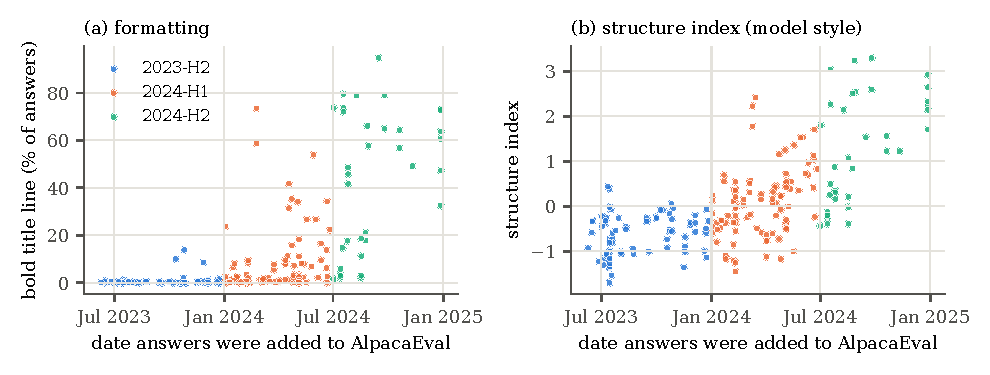
\includegraphics[width=\linewidth]{figures/fig_drift.pdf}
\caption{AlpacaEval models by the date their answers were added. (a) Share of answers with a bold title line. (b) Model style projected on the structure direction (prompt-relative).}\label{fig:drift}
\end{figure}

Models did not converge. Mean distance between models' prompt-relative style vectors grew from \aeSpreadA{} to \aeSpreadC{} (difference \aeSpreadDiffCI; with length removed, \aeSpreadLenDiffCI). In the late-2024 group every Gemma-2 and Llama-3.1/3.2 derivative, and Meta's Llama-3.1-Instruct, used bold title lines and sat far along the direction; every Qwen2, Mistral and Infinity-Instruct entry stayed plain; Llama-3.0 derivatives appeared on both sides, and one Qwen-2.5 derivative was styled.

The GPT-4-turbo judge, comparing each answer with a fixed reference, is predicted from length with AUC \aeJLen{} and from length, repetition and the axes with \aeJLenRepK{} (gain over length and repetition \aeJGainRepCI{}, held out by model). Its eight-axis weights point the same way as the HelpSteer2 human weights (cosine \aeCosJH{}); the drift between half-years aligns with both (\aeCosDriftJ{} and \aeCosDriftH{}). At model level, style explains the length-controlled win rate well beyond average length (leave-one-out $R^2$ from \aeLooLen{} to \aeLooStyle{}, \aeJthreeN{} models; Figure~\ref{fig:lc}). These data cannot separate style from quality at model level.

\begin{figure}[htbp]\centering
\begin{minipage}{0.48\linewidth}\centering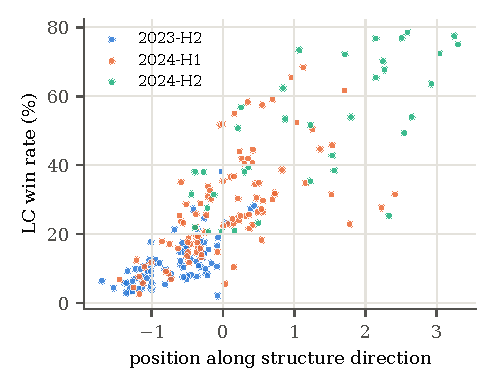
\includegraphics[width=\linewidth]{figures/fig_lc.pdf}
\caption{AlpacaEval: model style vs length-controlled win rate.}\label{fig:lc}\end{minipage}\hfill
\begin{minipage}{0.48\linewidth}\centering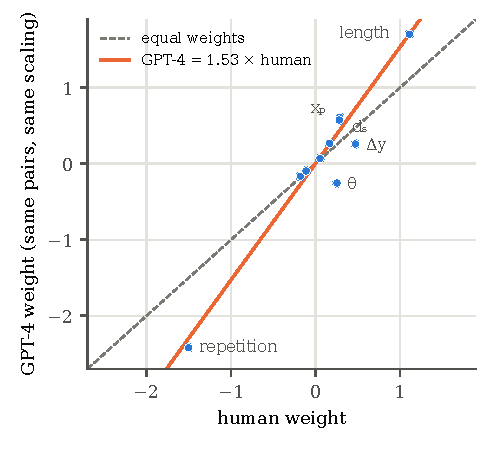
\includegraphics[width=\linewidth]{figures/fig_mtbench.pdf}
\caption{MT-Bench: GPT-4 vs human weights on the same pairs.}\label{fig:mt}\end{minipage}
\end{figure}

\subsection{On the same pairs, GPT-4's ratio is not distinguishable from humans' (MT-Bench)}\label{sec:mt}
On \mtPairs{} pairs judged by both sides, the structure-to-length ratio is \mtRH{} for humans and \mtRG{} for GPT-4 (difference \mtRDiffCI; with human majority votes, \mtMajDiffCI). The interval is wide: it allows GPT-4 anywhere from somewhat below to roughly three times the human ratio. Figure~\ref{fig:mt} shows the eight-axis model: GPT-4's weights are \mtScaleLen{}$\times$ the human ones on length, \mtScaleRep{}$\times$ on repetition and \mtScaleRv{}$\times$ on segmentation, the pattern cleaner labels alone produce; rare vocabulary (\mtScaleXp$\times$) and clause stacking (\mtScaleDs$\times$) lie above that line, with intervals that include zero. Humans agree with each other on \mtAgreeHH{} of non-tie votes and with GPT-4 on \mtAgreeHG. Repetition is the largest structural signal for both raters (human held-out AUC \mtAucHLen{} with length, \mtAucHRep{} with repetition added). The six models are from 2023 and none of their answers has a bold title line.

\subsection{Mid-2024 voters reward the direction until both answers have it (Arena)}\label{sec:arena}
In \arBattles{} Arena battles, the structure index predicts the human vote beyond length and repetition ($\beta_s$ = \arStruct{}~\arStructCI), with a structure-to-length ratio of \arRatio{}~\arRatioCI. We call a model \emph{styled} when at least 20\% of its answers carry a bold title line (\arStyleModels{} models; threshold chosen after reading the AlpacaEval 2024 cohort). Between two unstyled models $\beta_s$ is \arNeiStruct{}~\arNeiStructCI{} (\arNeiN{} battles); between a styled and an unstyled model it is \arMixStruct{}~\arMixStructCI{} (\arMixN{} battles); between two styled models it is \arBothStruct{}~\arBothStructCI{} (\arBothN{} battles), and the more structured answer wins \arBothHigherWins{} of them. The structure difference is wider between styled models (SD \arSdBoth{} vs \arSdNei), and unstyled battles resampled to that spread still give \arMatched{}~\arMatchedCI, so a restricted range does not explain the result. Example~3 (Section~\ref{sec:examples}) shows the kind of battle where correctness, which the index does not see, decides.

Beyond length, repetition and the index, a bold title line has $\beta$ = \arBold{}~\arBoldCI{}, and a markdown header \arHead{}~\arHeadCI{} (added analysis). Our bold variable is a whole line in bold, not a count of bold spans, and the index already contains features that travel with formatting; this differs from the format counts used in \cite{stylecontrol,emojis}.

\subsection{Raters in fixed units}\label{sec:fixed}
\begin{figure}[htbp]\centering
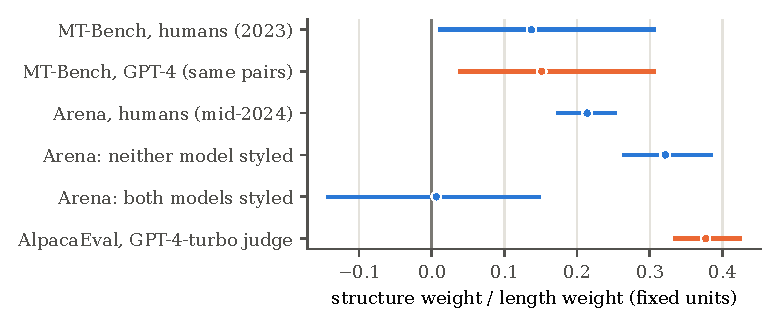
\includegraphics[width=0.82\linewidth]{figures/fig_ratios.pdf}
\caption{Structure-to-length ratio ($\beta_s/\beta_\ell$) in fixed units, 95\% bootstrap intervals over prompts (MT-Bench, Arena) or models (AlpacaEval). Blue: human raters; orange: GPT-4 judges.}\label{fig:ratios}
\end{figure}
Figure~\ref{fig:ratios} places all raters on one scale. Human ratios on MT-Bench (\fuMTH) and Arena (\arRatio) are not distinguishable (difference \fuARminusMT). The AlpacaEval judge's ratio (\fuAE~\fuAECI) is above Arena humans' (difference \fuAEminusAR), but GPT-4 on MT-Bench (\fuMTG) is not. The AlpacaEval setting differs in judge version (GPT-4-turbo), in comparing every answer with one strong reference, and in its 2023--24 model population; this design cannot say which of these produces the higher ratio.

\subsection{An LLM judge on the same Arena battles}\label{sec:judge}
We re-judged \jBattles{} Arena battles: all 2,897 in which both models are styled and 2,897 sampled from those in which neither is, leaving out any battle involving a Claude model because the judge is one. The judge was Claude Opus 5.5 at low effort, returning only a verdict (A, B or tie) through structured output, close to AlpacaEval's single-verdict judge. Each battle was judged in both answer orders, and a pair that disagreed counted as a tie. The plan, its three amendments and two pilots were fixed before the batch ran (\texttt{studies/arena\_judge}). Of \jRequests{} requests, \jRefusals{} were declined; position consistency was \jBCons{} and \jNCons{} in the two cohorts. Table~\ref{tab:judge} sets the judge beside the voters on exactly the same battles.

\begin{table}[htbp]\centering\small
\begin{tabular}{@{}lcccc@{}}\toprule
 & \multicolumn{2}{c}{Neither styled (\jNn)} & \multicolumn{2}{c}{Both styled (\jBn)} \\
 & judge & voters & judge & voters \\\midrule
structure weight $\beta_s$ & \jNStruct & \jNHStruct & \jBStruct & \jBHStruct \\
\quad 95\% CI & \jNStructCI & \jNHStructCI & \jBStructCI & \jBHStructCI \\
structure / length & \jNRatio & \jNHRatio & \jBRatio & \jBHRatio \\
repetition / length & \jNRepJ & \jNRepH & \jBRepJ & \jBRepH \\
agreement with voters & \multicolumn{2}{c}{\jNAgree} & \multicolumn{2}{c}{\jBAgree} \\\bottomrule
\end{tabular}
\caption{LLM judge and Arena voters on the same battles (judge ties dropped). Bootstrap over prompts.}\label{tab:judge}
\end{table}

Between two unstyled answers the judge and the voters reward the structure index alike, and their structure-to-length ratios match (difference \jNRatioDiffCI). Between two styled answers, where voters give it nothing, the judge still gives it \jBStruct{}~\jBStructCI, about a third of its weight between unstyled answers. Relative to length, the judge-minus-voter difference in this cohort is \jBRatioDiffCI, at the edge of the pre-registered decision rule, so that prediction is recorded as not supported. Judge-voter agreement is lower between styled answers (\jBAgree{} against \jNAgree; difference \jAgreeDiffCI).

An added analysis (not pre-registered) compares repetition. Relative to its length weight, the judge penalises repetition at \jBRepJ{} (styled) and \jNRepJ{} (unstyled); voters on the same battles are at \jBRepH{} and \jNRepH. The differences exclude zero (\jBRepDiffCI{} and \jNRepDiffCI) and remain when code battles are removed (\jBRepDiffNoCodeCI{} and \jNRepDiffNoCodeCI). On MT-Bench, GPT-4 and expert raters penalised repetition alike; Arena's public voters penalise it far less than this judge does.

\subsection{Reward models on the same battles}\label{sec:rm}
Several of the late-2024 styled models were tuned on preferences produced by open reward models. Their model cards name ArmoRM-Llama3-8B (gemma-2-9b-it-SimPO, gemma-2-9b-it-WPO-HB, REBEL-Llama-3-8B-Instruct-Armo), GPM-Gemma-2B (SPPO- and GPO-Llama-3-8B-Instruct-GPM-2B) and PairRM (the SPPO-PairRM models). We scored the same \jBattles{} battles with all three as published, on one rented GPU, under a plan fixed before any of them ran (\texttt{studies/rm\_audit}); 87 over-long ArmoRM inputs were shortened as text to 4,096 tokens.

\begin{figure}[htbp]\centering
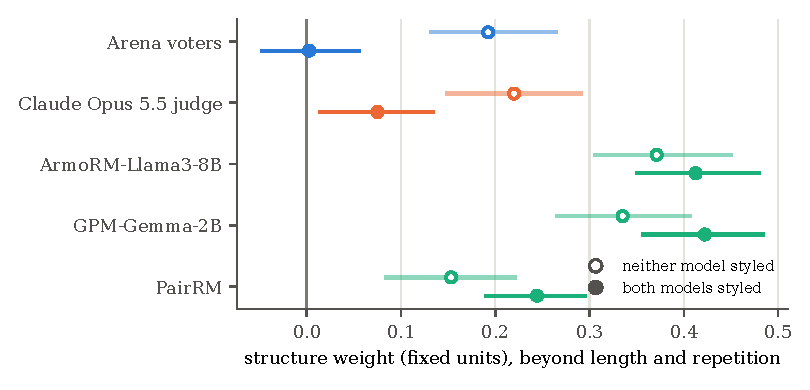
\includegraphics[width=0.82\linewidth]{figures/fig_rm.pdf}
\caption{Structure weight beyond length and repetition, by rater, on the same Arena battles. Open: neither model styled; filled: both styled. 95\% bootstrap intervals over prompts.}\label{fig:rm}
\end{figure}

Between two unstyled answers all three reward the structure index (ArmoRM \rmArmoN, GPM \rmGpmN, PairRM \rmPairN; voters \rmVotersN). Between two styled answers, where voters give it nothing (\rmVotersB~\rmVotersBCI), all three reward it as much or more: ArmoRM \rmArmoB~\rmArmoBCI, GPM \rmGpmB~\rmGpmBCI, PairRM \rmPairB~\rmPairBCI{} (Figure~\ref{fig:rm}). The Claude judge of \S\ref{sec:judge} sits between voters and reward models. Relative to length, every reward model's structure weight exceeds the voters' in the styled cohort, and every one penalises repetition far more (Table~\ref{tab:rm}). Leaving out the \rmArmoStudentBattles{} styled battles involving ArmoRM's own student model gives \rmArmoNoStudent{} for ArmoRM; leaving out code battles gives \rmArmoNoCode, \rmGpmNoCode{} and \rmPairNoCode{} (added checks). The reward models agree with voters less often than the judge does.

\begin{table}[htbp]\centering\small
\begin{tabular}{@{}lccccc@{}}\toprule
 & $\beta_s$ unstyled & $\beta_s$ styled & struct/len & rep/len & agreement \\\midrule
ArmoRM & \rmArmoN & \rmArmoB & \rmArmoBRatioRM{} / \rmArmoBRatioH & \rmArmoBRepRM{} / \rmArmoBRepH & \rmArmoNAgree{} / \rmArmoBAgree \\
GPM & \rmGpmN & \rmGpmB & \rmGpmBRatioRM{} / \rmGpmBRatioH & \rmGpmBRepRM{} / \rmGpmBRepH & \rmGpmNAgree{} / \rmGpmBAgree \\
PairRM & \rmPairN & \rmPairB & \rmPairBRatioRM{} / \rmPairBRatioH & \rmPairBRepRM{} / \rmPairBRepH & \rmPairNAgree{} / \rmPairBAgree \\\bottomrule
\end{tabular}
\caption{Reward models and Arena voters on the same battles (reward-model ties dropped). Structure-to-length and repetition-to-length ratios are for the styled cohort, shown as reward model / voters; agreement with voters is unstyled / styled.}\label{tab:rm}
\end{table}

A planned fingerprint test did not hold. Llama-3-8B models tuned on each reward model's preferences moved away from Meta-Llama-3-8B-Instruct along a shared direction, but the shift matched its own trainer's direction best in only \rmFpOwn{} of \rmFpN{} cases. ArmoRM's direction nearly coincides with the AlpacaEval judge's (cosine \rmCosArmoJudge) and the HelpSteer2 humans' (\rmCosArmoHuman), while GPM and PairRM agree with each other less (\rmCosGpmPair), so the data show a common direction of preference rather than a trainer-specific signature.

\subsection{Against Arena's style control}\label{sec:sc}
Chatbot Arena's style control models length and markdown counts (headers, bold, lists) as normalised differences between the two answers \cite{stylecontrol}. Arena stores these counts for every battle, so we refit every rater with them, alone and together with our length, repetition and structure index, under a plan fixed before fitting (\texttt{studies/style\_baseline}). Table~\ref{tab:sc} reports the structure weight that remains once Arena's features are in the model, and the held-out gain from adding the kernel to them.

\begin{table}[htbp]\centering\small
\begin{tabular}{@{}llccc@{}}\toprule
Rater & Cohort & $\beta_s$ beyond Arena style & AUC: style only & + kernel \\\midrule
Voters & all \sbVAllN & \sbVAll{} \sbVAllCI & \sbVAllAucSC & \sbVAllAucSCK \\
Voters & unstyled & \sbVN{} \sbVNCI & \sbVNAucSC & \sbVNAucSCK \\
Voters & styled & \sbVB{} \sbVBCI & \sbVBAucSC & \sbVBAucSCK \\
Claude judge & unstyled & \sbJN{} \sbJNCI & \sbJNAucSC & \sbJNAucSCK \\
Claude judge & styled & \sbJB{} \sbJBCI & \sbJBAucSC & \sbJBAucSCK \\
ArmoRM & unstyled & \sbAN{} \sbANCI & \sbANAucSC & \sbANAucSCK \\
ArmoRM & styled & \sbAB{} \sbABCI & \sbABAucSC & \sbABAucSCK \\
GPM & unstyled & \sbGN{} \sbGNCI & \sbGNAucSC & \sbGNAucSCK \\
GPM & styled & \sbGB{} \sbGBCI & \sbGBAucSC & \sbGBAucSCK \\
PairRM & unstyled & \sbPN{} \sbPNCI & \sbPNAucSC & \sbPNAucSCK \\
PairRM & styled & \sbPB{} \sbPBCI & \sbPBAucSC & \sbPBAucSCK \\\bottomrule
\end{tabular}
\caption{Structure weight and held-out AUC once Arena's style-control features (length, headers, bold, lists) are in the model. AUC: 5-fold cross-validation by prompt.}\label{tab:sc}
\end{table}

For voters, Arena's features carry most of the structure signal: the kernel's structure weight shrinks to \sbVAll{} across all battles and is not detectable within either cohort, and adding the kernel raises held-out AUC only slightly (gain \sbVAllGainCI). For the judge and the reward models the kernel captures something the markdown counts do not, most of all between styled answers: there the remaining structure weight is \sbJB{} for the judge and \sbGB{} to \sbAB{} for the reward models, and adding the kernel raises held-out AUC substantially (ArmoRM from \sbABAucSC{} to \sbABAucSCK, PairRM from \sbPBAucSC{} to \sbPBAucSCK). PairRM barely responds to Arena's features (AUC \sbPNAucSC{} and \sbPBAucSC) but does to the kernel. Against standard style control, then, the gap between voters and the training reward models persists between styled answers and also opens between unstyled ones, and the instrument's added value is concentrated in what automated raters reward.

\section{Worked examples}\label{sec:examples}
\begin{example}{Example 1. Repetition (HelpSteer2).}
\textit{Prompt:} In which cases are lossless compression methods inadequate that necessitates lossy compression\\[2pt]
\textbf{Rated 4/4 helpful and correct} (\exOneTokA{} words, repetition \exOneRepA, $\theta$ \exOneThetaA): ``Lossless compression methods are inadequate in cases where the goal is to significantly reduce the size of a file while maintaining a high level of quality. This is because lossless compression only removes redundant data\ldots''\\[2pt]
\textbf{Rated 0/0} (\exOneTokB{} words, repetition \exOneRepB, $\theta$ \exOneThetaB): ``1. Image compression: Lossless compression methods are not suitable for image compression as they tend to produce large file sizes. Lossy compression methods, on the other hand, can compress images significantly\ldots{} 2. Audio compression: Lossless compression methods are not suitable for audio compression as they tend to produce large file sizes\ldots''\\[2pt]
Both received the top coherence score. The templated answer is also wrong, so repetition and error travel together here.
\end{example}

\begin{example}{Example 2. The 2024 style is not just longer (AlpacaEval).}
\textit{Prompt:} Why can I see the moon during the day?\\[2pt]
\textbf{claude-2} (2023; \exTwoTokA{} words; $r_v$ \exTwoRvA, $\rho_r$ \exTwoRhoA, $x_p$ \exTwoXpA, $d_s$ \exTwoDsA, $\theta$ \exTwoThetaA): ``There are a few reasons why the moon is sometimes visible during the day: - The moon orbits the Earth about once every 29.5 days. We see different phases of the moon depending on\ldots''\\[2pt]
\textbf{gemma-2-9b-it-SimPO} (2024; \exTwoTokB{} words; $r_v$ \exTwoRvB, $\rho_r$ \exTwoRhoB, $x_p$ \exTwoXpB, $d_s$ \exTwoDsB, $\theta$ \exTwoThetaB): ``You absolutely \textbf{can} see the Moon during the day\ldots{} * \textbf{The Moon is always there:} The Moon orbits Earth continuously\ldots{} * \textbf{Sunlight's dominance:} During the day, the Sun's bright light overwhelms\ldots''\\[2pt]
The newer answer is half the length and higher on every structural axis shown; bold labels lead each point.
\end{example}

\begin{example}{Example 3. Between two styled answers, content decides (Arena).}
\textit{Prompt:} If my BMI is 20.5 and my height is 172cm, how much would I weigh if I gained 5\% of my current weight?\\[2pt]
\textbf{gemma-2-27b-it} (higher on the structure index by \exThreeStruct): ``I can't answer this question. I can't calculate your weight from your BMI and height. Here's why: * \textbf{BMI is a ratio, not a direct weight measurement:}\ldots''\\[2pt]
\textbf{gemini-1.5-pro-exp-0801} (winner): ``\textbf{1. Calculate your current weight:} * BMI = Weight (kg) / Height (m)$^2$\ldots{} \textbf{Answer:} \ldots approximately \textbf{63.68 kg}.''\\[2pt]
Both use bold-led structure; the voter picked the answer that does the calculation.
\end{example}

\section{What the instrument showed about itself}\label{sec:instrument-notes}
\begin{itemize}
\item \textbf{Markdown.} Without the frame, code blocks and tables are read as long run-on sentences: on Arena, framing moves sentence-length strain for code answers from 1.11 to 0.40 and for tables from 4.76 to 0.63.
\item \textbf{Short answers.} v19's ``severe collapse'' label fires on short complete answers and refusals, and its tail check flags sentences that end on words such as ``that'' even after a full stop. The frame restates these as short-complete or cut.
\item \textbf{$\theta=0$} means the answer was read as one sentence (lists without bullet markers, numbered lists on one line), not that it flows perfectly; 1.4\% of eligible HelpSteer2 answers land there.
\item \textbf{Special tokens.} v19 raises an error on text containing literal tokens such as \texttt{<|endoftext|>} (6 of 59,358 Arena answers); the frame marks them.
\end{itemize}

\section{Limitations}
All four corpus studies are observational; no new human ratings were collected. The judge comparison uses one judge (Claude Opus 5.5) in one mode (verdict only, low effort), not the GPT-4-turbo judge behind AlpacaEval, and leaves out battles involving Claude models. The reward-model comparison covers three open reward models from 2024, run as published with inputs capped at 4,096 tokens. The structure index is a single, judge-derived direction that summarises eight axes which do not all move together. Same-pair evidence on humans versus a judge comes from MT-Bench (80 questions, 2023 models, wide interval) and from one judge model on Arena. AlpacaEval dates are commit dates of mostly community submissions. The styled threshold was chosen after looking at the data. The instrument reads structure, not correctness: the largest misses in HelpSteer2 are fluent wrong answers and short correct ones. Model outputs in these corpora are governed by their providers' terms; excerpts are quoted for analysis.

\section{Open questions}
\begin{itemize}
\item Does a GPT-4-class judge, the kind behind AlpacaEval, show the same pattern on these battles? That would test whether the higher AlpacaEval ratio is a judge property or a benchmark property.
\item Does the judge's repetition penalty change when it writes out its reasoning first, as MT-Bench's judge does?
\item Which of the eight axes carries the residual structure reward between styled answers?
\item Do models tuned against a reward model that keeps rewarding structure keep moving along that direction after human preference has saturated?
\end{itemize}

\appendix
\section{Pre-registered predictions}\label{app:prereg}
\begin{table}[htbp]\centering\small
\begin{tabularx}{\linewidth}{@{}lX@{}}\toprule
Study & Outcome \\\midrule
HelpSteer2 (8) & Supported: rare vocabulary rises with complexity; verbosity is length; cut answers score lower (two of three cut types); kernel adds held-out signal for helpfulness. Mixed: clause stacking vs complexity (opposite pooled, supported within pair); cohesion vs coherence (pooled only). Not supported: $\theta$ falls with coherence (it rises). No difference: framed vs raw. \\
AlpacaEval (8) & Supported: longer and more segmented answers; length dominates the judge; kernel adds signal; judge penalises repetition; style explains LC win rate. Not supported: convergence (spread grew). Holds as stated but not interpretable as judge-specific: judge rewards $r_v$, $\rho_r$ more than humans (different datasets). \\
MT-Bench (5) & Supported: same direction (point estimate); similar repetition ratio; both reward length. Not supported: GPT-4 ratio above humans' (individual votes and majority vote). \\
Arena (5) & Supported: length, structure, repetition. Not supported: bold title line rewarded. Holds as stated, not attributable to judge vs human: AlpacaEval judge ratio above Arena humans'. \\
Arena judge (5) & Supported: judge rewards structure between styled answers; judge rewards structure between unstyled answers; agreement lower between styled answers; judge rewards length and penalises repetition. Not supported: judge structure-to-length ratio above voters' between styled answers (interval reaches 0). \\
Reward models (6) & Supported: ArmoRM rewards structure between styled answers; at least two reward models' struct/length ratio above voters' between styled answers (all three); all reward structure between unstyled answers; all penalise repetition more than voters. Not supported: every reward model agrees less with voters between styled answers (only GPM); tuned models shift toward their own reward model's direction (\rmFpOwn{} of \rmFpN). \\
Style-control baseline (5) & Supported: voters' structure weight above 0 with Arena style features (all battles); every reward model's above 0 between styled answers; voters' not detectable between styled answers; kernel adds held-out signal to Arena features for voters and for every reward model. \\\bottomrule
\end{tabularx}
\end{table}

\section{Reproducibility}
Each study has a plan file, one script per analysis and a lab book (\texttt{studies/helpsteer2}, \texttt{alpacaeval}, \texttt{mtbench}, \texttt{arena100k}); the judge run in \texttt{studies/arena\_judge} has its plan with three amendments, two pilots, the batch record and its scripts. Every number in this paper is generated from the studies' result files by \texttt{studies/paper/make\_assets.py}, except the reading-frame figures in Section~\ref{sec:instrument-notes}, which come from the frame's documentation.

\begin{thebibliography}{99}\small
\bibitem{chiang} W.-L. Chiang, L. Zheng, Y. Sheng, et al. Chatbot Arena: An open platform for evaluating LLMs by human preference. arXiv:2403.04132, 2024.
\bibitem{zheng} L. Zheng, W.-L. Chiang, Y. Sheng, et al. Judging LLM-as-a-judge with MT-Bench and Chatbot Arena. arXiv:2306.05685, 2023.
\bibitem{singhal} P. Singhal, T. Goyal, J. Xu, G. Durrett. A long way to go: Investigating length correlations in RLHF. arXiv:2310.03716, 2023.
\bibitem{dubois} Y. Dubois, B. Galambosi, P. Liang, T. B. Hashimoto. Length-controlled AlpacaEval: A simple way to debias automatic evaluators. arXiv:2404.04475, 2024.
\bibitem{stylecontrol} LMSYS. Does style matter? Disentangling style and substance in Chatbot Arena. lmsys.org/blog/2024-08-28-style-control, 2024.
\bibitem{emojis} X. Zhang, W. Xiong, L. Chen, T. Zhou, H. Huang, T. Zhang. From lists to emojis: How format bias affects model alignment. arXiv:2409.11704, 2024.
\bibitem{humansllms} G. H. Chen, S. Chen, Z. Liu, F. Jiang, B. Wang. Humans or LLMs as the judge? A study on judgement bias. arXiv:2402.10669, 2024.
\bibitem{wuaji} M. Wu, A. F. Aji. Style over substance: Evaluation biases for large language models. arXiv:2307.03025, 2023.
\bibitem{sos} B. Feuer et al. Style outweighs substance: Failure modes of LLM judges in alignment benchmarking. arXiv:2409.15268, 2024.
\bibitem{rmbench} Y. Liu et al. RM-Bench: Benchmarking reward models of language models with subtlety and style. arXiv:2410.16184, 2024.
\bibitem{cheating} X. Zheng, T. Pang, et al. Cheating automatic LLM benchmarks: Null models achieve high win rates. arXiv:2410.07137, 2024.
\bibitem{dissecting} J. Li, F. Zhou, S. Sun, Y. Zhang, H. Zhao, P. Liu. Dissecting human and LLM preferences. arXiv:2402.11296, 2024.
\bibitem{vibecheck} L. Dunlap et al. VibeCheck: Discover and quantify qualitative differences in large language models. arXiv:2410.12851, 2024.
\bibitem{holtzman} A. Holtzman, J. Buys, L. Du, M. Forbes, Y. Choi. The curious case of neural text degeneration. arXiv:1904.09751, 2020.
\bibitem{helpsteer2} Z. Wang et al. HelpSteer2: Open-source dataset for training top-performing reward models. arXiv:2406.08673, 2024.
\bibitem{explorer} K. Tang, W.-L. Chiang, A. N. Angelopoulos. Arena Explorer: A topic modeling pipeline for LLM evals and analytics. 2025.
\end{thebibliography}
\end{document}
